% =====================================================================
% Project #11 report -- Week 2 progress: Introduction, Methods, Results.
% IEEE conference template. Compile with pdflatex (Overleaf: upload as-is).
% =====================================================================
\IfFileExists{IEEEtran.cls}{%
  \documentclass[conference]{IEEEtran}
  \newcommand{\usingieee}{}
}{%
  \documentclass[10pt,twocolumn]{article}
  \usepackage[letterpaper,top=0.75in,bottom=1in,left=0.625in,right=0.625in,columnsep=0.25in]{geometry}
  \usepackage{mathptmx}
  \usepackage[font=footnotesize]{caption}
}
\usepackage{amsmath,amssymb}
\usepackage{booktabs}
\usepackage[noadjust]{cite}
\usepackage[hidelinks]{hyperref}
\usepackage{tikz}
\usepackage{graphicx}
\usetikzlibrary{quantikz}

\begin{document}

\ifdefined\usingieee
\title{Does a Variational Quantum Head Help in the Small-Data Regime?
A Controlled Study of Hybrid Transfer Learning for Chest X-Ray Classification}
\author{\IEEEauthorblockN{Ali Arslan}
\IEEEauthorblockA{MS Artificial Intelligence, Lahore University of Management Sciences (LUMS)\\
Quantum Machine Learning, Fall 2026 --- Project \#11}}
\maketitle
\else
\title{\vspace{-1.2em}\Large\bfseries Does a Variational Quantum Head Help in the Small-Data Regime?
A Controlled Study of Hybrid Transfer Learning for Chest X-Ray Classification}
\author{Ali Arslan\\ \small MS Artificial Intelligence, Lahore University of Management Sciences (LUMS)\\
\small Quantum Machine Learning, Fall 2026 --- Project \#11}
\date{\vspace{-2em}}
\maketitle
\fi

\begin{abstract}
Hybrid transfer learning places a small variational quantum circuit (VQC)
on top of a frozen, pretrained convolutional network. Such quantum heads are
often claimed to be especially useful when labeled data are scarce. We test
this claim on pediatric chest X-ray classification (PneumoniaMNIST). A frozen
ResNet-18 produces image features, which are reduced to $d\in\{4,8\}$
dimensions and passed to one of three heads: a linear head, a
parameter-matched multilayer perceptron (MLP), or a VQC. All heads receive
identical features, data subsamples, loss, optimizer, and tuning budget. We
vary the number of labeled training images from 50 to 1{,}000 and evaluate
the trained VQC on ideal, noisy, and real IBM quantum backends. The
criterion that would falsify the small-data claim is fixed before any
quantum result is observed. At $d=4$ the VQC is statistically equivalent
to the matched MLP at $n\le100$, which falsifies the small-data claim. At
$d=8$ it exceeds the MLP at $n=50$ and $100$ under the same test, largely
because the classical heads become unstable, and the advantage disappears
by $n=250$. Removing entanglement lowers AUROC at every training size.
Under simulated depolarizing noise, AUROC is preserved while accuracy at a
fixed threshold collapses. Hardware results will follow.
\end{abstract}

% =====================================================================
\section{Introduction}
Medical image classification is a natural testbed for data-efficient
learning: expert labels are expensive, and many clinical tasks have only
hundreds of labeled examples. Transfer learning addresses this by reusing a
network pretrained on a large generic dataset as a fixed feature extractor
and training only a small classification head on the target
task~\cite{he2016}.

Quantum machine learning (QML) proposes replacing such a head with a
\emph{variational quantum circuit} (VQC): a parameterized sequence of
quantum gates whose measured expectation values serve as model
outputs~\cite{cerezo2021}. Mari \emph{et al.}~\cite{mari2020} formalized this
idea as \emph{classical-to-quantum transfer learning}. A pretrained
ResNet-18 produces features, a small linear layer compresses them to a few
numbers, and a 4-qubit VQC classifies them. Because current quantum
processors offer only a few reliable qubits, this hybrid design is one of
the few ways to apply VQCs to realistic image data.

A recurring claim in this literature is that quantum heads are
particularly advantageous when training data are limited. Medical-imaging
studies frequently report hybrid models outperforming classical
ones~\cite{shahjalal2025}. However, the evidence is fragile. In a large-scale
benchmark of 12 QML models across 160 datasets, Bowles
\emph{et al.}~\cite{bowles2024} found that out-of-the-box classical models
systematically outperformed the quantum models, and that hybrid models
performed similarly to their purely classical hosts. Kölle
\emph{et al.}~\cite{kolle2024} showed that in hybrid transfer learning, the
classical components drive much of the classification performance, and
that this contribution is often mistakenly attributed to the quantum part.
Schuld and Killoran~\cite{schuldkilloran2022} argue more broadly that the
field's focus on ``beating'' classical machine learning has encouraged weak
comparisons. Most recently, Martín-Pérez \emph{et al.}~\cite{martinperez2026}
compared quantum and classical heads on several frozen backbones, including
one medical dataset and IBM hardware. Their classical baseline was not
parameter-matched, however, and the amount of training data was never
varied. The small-data claim therefore remains largely untested.

\textbf{Research question.} \emph{Does a VQC head on top of a frozen
pretrained CNN help on a small medical-image task compared with a classical
head of matched size?}

\textbf{Contribution.} We do not propose a new architecture. Our
contribution is a controlled \emph{learning-curve} comparison, designed so
that any of the three possible outcomes (quantum better, equivalent, or
worse) is informative:
\begin{enumerate}
\item quantum and classical heads receive identical features, identical
training subsamples, and comparable parameter budgets (26 vs.\ 25 for
$d=4$; 50 vs.\ 51 for $d=8$);
\item the number of labeled images is varied from 50 to 1{,}000, with
repeated stratified subsamples and paired comparisons;
\item the falsification criterion for the small-data claim is fixed in
advance (Sec.~\ref{sec:stats});
\item the trained VQC is evaluated on exact, finite-shot, noisy-simulated,
and real IBM quantum backends, and ablations isolate the role of
entanglement and circuit depth.
\end{enumerate}

\textbf{Hypothesis.} At $n\le100$ training images, the VQC head achieves
higher test AUROC than the parameter-matched MLP head, and this gap shrinks
as $n$ grows. A finding that the classical head performs as well or better
is a valid outcome of this study.

% =====================================================================
\section{Methods}

\subsection{Dataset}
We use PneumoniaMNIST from MedMNIST v2~\cite{yang2023}. It is derived from
5{,}856 pediatric chest X-rays~\cite{kermany2018} labeled for binary
classification (pneumonia, positive class, vs.\ normal). We use the official
splits: 4{,}708 training, 524 validation, and 624 test images. The classes
are imbalanced, with about 74\% of training images showing pneumonia. We
use the $224\times224$ MedMNIST+ release, which is derived directly from the
source images and matches ResNet-18's native input resolution. This avoids
upsampling the standard $28\times28$ images.

\subsection{Training subsamples}
\label{sec:folds}
To study data efficiency, we train on $n\in\{50,100,250,500,1000\}$
labeled images. For each $n$, we draw $K=5$ stratified subsamples from the
training split, each preserving the class ratio of the full split. Every
subsample $(n,k)$ is generated from a deterministic seed, and its indices
are saved and version-controlled. Every head is trained on exactly the same
subsamples, so all comparisons are paired. The validation and test sets are
fixed across all runs.

\subsection{Feature extraction}
Grayscale images are replicated to three channels and normalized with
ImageNet channel statistics. They are passed through an ImageNet-pretrained
ResNet-18~\cite{he2016} whose final classification layer is removed. The
output of the global average-pooling layer gives a feature vector
$\mathbf{u}\in\mathbb{R}^{512}$ per image. The backbone is frozen: no
weights are updated, and features are computed once and cached.

\subsection{Dimensionality reduction and angle scaling}
A 4- to 8-qubit circuit can accept only 4 to 8 inputs, so the 512-d
features are reduced by principal component analysis (PCA) to
$d\in\{4,8\}$ components. PCA is fit on the 4{,}708 training images only,
without labels; validation and test images never influence the fit. Each
component $z_j$ is then mapped linearly to an angle using the 1st and 99th
percentiles $(\ell_j,h_j)$ of the training split, with clipping:
\begin{equation}
x_j=\frac{\pi}{2}\left(2\,\frac{\mathrm{clip}(z_j,\ell_j,h_j)-\ell_j}{h_j-\ell_j}-1\right)
\in\left[-\tfrac{\pi}{2},\tfrac{\pi}{2}\right].
\end{equation}
Using percentiles rather than the minimum and maximum prevents a few
extreme images from compressing the range for all others. \emph{All} heads,
quantum and classical, receive the same vector
$\mathbf{x}\in[-\pi/2,\pi/2]^d$.

\subsection{Classification heads}
Each head maps $\mathbf{x}$ to a single logit $f(\mathbf{x})$; the
predicted probability of pneumonia is $\sigma(f(\mathbf{x}))$.

\textbf{Linear head:} $f(\mathbf{x})=\mathbf{w}^\top\mathbf{x}+b$, with $d+1$
parameters.

\textbf{MLP head (parameter-matched):}
$f(\mathbf{x})=\mathbf{v}^\top\mathrm{ReLU}(W\mathbf{x}+\mathbf{c})+b$,
with $h$ hidden units and $(d+2)h+1$ parameters. We use $h=4$ for $d=4$
(25 parameters) and $h=5$ for $d=8$ (51 parameters), the closest matches to
the VQC.

\textbf{VQC head:} The circuit acts on $d$ qubits, one per feature, all
initialized in $\lvert0\rangle$ (Fig.~\ref{fig:circuit}).
\begin{enumerate}
\item \emph{Angle encoding.} Feature $x_i$ sets a rotation about the
$y$-axis of qubit $i$:
\begin{equation}
R_Y(x_i)\lvert0\rangle=\cos\tfrac{x_i}{2}\lvert0\rangle+\sin\tfrac{x_i}{2}\lvert1\rangle,
\end{equation}
giving the product state
$\lvert\psi(\mathbf{x})\rangle=\bigotimes_{i=1}^{d}R_Y(x_i)\lvert0\rangle$.
\item \emph{Variational layers.} Each of $L=2$ layers applies a trainable
single-qubit rotation
$W(\boldsymbol{\theta}_{l,i})=R_Y(\theta_{l,i,3})R_Z(\theta_{l,i,2})R_Y(\theta_{l,i,1})$
to every qubit. A ring of CNOT gates
($1\!\to\!2\!\to\!\dots\!\to\!d\!\to\!1$) follows, entangling neighboring
qubits. The full unitary is
\begin{equation}
U(\boldsymbol{\theta})=\prod_{l=1}^{L}\Big[E_{\mathrm{ring}}\bigotimes_{i=1}^{d}W(\boldsymbol{\theta}_{l,i})\Big].
\end{equation}
\item \emph{Readout.} We measure the Pauli-$Z$ expectation of every qubit
and average:
\begin{equation}
f(\mathbf{x})=\alpha\,\frac{1}{d}\sum_{i=1}^{d}
\langle\psi(\mathbf{x})\rvert U^\dagger(\boldsymbol{\theta})\,Z_i\,U(\boldsymbol{\theta})\lvert\psi(\mathbf{x})\rangle+\beta,
\end{equation}
where $\alpha$ and $\beta$ are trainable. Each expectation lies in
$[-1,1]$, and $\alpha,\beta$ map it to the logit scale.
\end{enumerate}
The VQC has $3dL+2$ trainable parameters: 26 for $d=4$ and 50 for $d=8$.
Angles are initialized from $\mathcal{N}(0,0.1^2)$. Small initial angles
keep the circuit close to identity, which mitigates the vanishing-gradient
(barren-plateau) problem~\cite{mcclean2018}. The circuit is simulated
exactly with PennyLane's \texttt{default.qubit}~\cite{bergholm2018}, and
gradients are obtained by backpropagation through the simulator.

\emph{Deviation from the synopsis:} the synopsis specified the readout
$\langle Z_1\rangle$ alone. We changed it to the mean over all qubits
before any results were obtained. Without entanglement, $\langle Z_1\rangle$
depends only on $x_1$, which would make the no-entanglement ablation
degenerate. Averaging keeps every feature in play for both variants, at no
extra parameters.

\begin{figure}[t]
\centering
\ifdefined\quantikz
\resizebox{\columnwidth}{!}{%
\begin{quantikz}[row sep=0.2cm, column sep=0.25cm]
\lstick{$\ket{0}$} & \gate{R_Y(x_1)} & \gate{W(\boldsymbol\theta_{l,1})}\gategroup[4,steps=5,style={dashed,rounded corners,inner xsep=2pt},label style={label position=below,anchor=north,yshift=-0.2cm}]{repeated $L=2$ times} & \ctrl{1} & \qw & \qw & \targ{} & \meter{} \\
\lstick{$\ket{0}$} & \gate{R_Y(x_2)} & \gate{W(\boldsymbol\theta_{l,2})} & \targ{} & \ctrl{1} & \qw & \qw & \meter{} \\
\lstick{$\ket{0}$} & \gate{R_Y(x_3)} & \gate{W(\boldsymbol\theta_{l,3})} & \qw & \targ{} & \ctrl{1} & \qw & \meter{} \\
\lstick{$\ket{0}$} & \gate{R_Y(x_4)} & \gate{W(\boldsymbol\theta_{l,4})} & \qw & \qw & \targ{} & \ctrl{-3} & \meter{}
\end{quantikz}}
\else
\fbox{VQC circuit diagram (requires the \texttt{quantikz} package)}
\fi
\caption{VQC head for $d=4$. Features are angle-encoded with $R_Y$. Each
layer applies trainable rotations $W=R_YR_ZR_Y$ and a CNOT ring. The output
is the mean of the four $\langle Z_i\rangle$, rescaled by trainable
$\alpha,\beta$.}
\label{fig:circuit}
\end{figure}

\textbf{Reference model (not a competitor):} logistic regression on all 512
standardized ResNet features (inverse regularization $C$ chosen on
validation). It shows how much information the reduction to $d$ dimensions
discards.

\subsection{Training protocol}
All heads are trained by an identical procedure. Because $n\le1000$, every
optimizer step uses the full training subsample. We use Adam~\cite{kingma2015}
to minimize class-weighted binary cross-entropy, with the positive class
weighted by $n_{\mathrm{neg}}/n_{\mathrm{pos}}$ so that the majority class
does not dominate. Training runs for at most 1000 epochs. It stops early
when the validation loss has not improved for 50 epochs, and the weights
with the lowest validation loss are restored. Each head receives the same
hyperparameter search: learning rate $\in\{0.01,0.03,0.1,0.3\}$ $\times$ weight
decay $\in\{0,10^{-3}\}$. The configuration with the highest validation
AUROC is selected. Each $(n,\text{subsample})$ pair is trained with 3
initialization seeds, giving 15 runs per head and setting. The test set is
never used for training, early stopping, or model selection.


\emph{Deviation from the synopsis:} after the Week~1 pilot, the epoch
limit was raised from 300 to 1000, patience from 30 to 50, and 0.3 was
added to the learning-rate grid, because many runs had stopped at the
epoch limit rather than by early stopping. The change was applied to all
heads before the full quantum grid was run, and it moved mean validation
AUROC by at most 0.003.

\subsection{Gradient verification}
On hardware, gradients cannot be obtained by backpropagation. They are
instead computed with the parameter-shift rule~\cite{mitarai2018,schuld2019}:
for a gate $e^{-i\theta P/2}$ with Pauli generator $P$,
\begin{equation}
\frac{\partial\langle Z\rangle}{\partial\theta}=
\tfrac{1}{2}\Big[\langle Z\rangle_{\theta+\pi/2}-\langle Z\rangle_{\theta-\pi/2}\Big],
\end{equation}
which is exact rather than a finite-difference approximation. Before any
experiment, we verify that the simulator's backpropagation gradients agree
with parameter-shift gradients to within $10^{-5}$ for $d=4$ and $d=8$.

\subsection{Evaluation and falsification criterion}
\label{sec:stats}
The primary metric is test AUROC, which does not depend on a threshold and
is robust to class imbalance. We also report AUPRC, accuracy, balanced
accuracy, F1, sensitivity, and specificity. For these, the decision
threshold maximizes Youden's $J$ (sensitivity $+$ specificity $-1$) on the
\emph{validation} set~\cite{youden1950}.

For each $(n,d)$, the paired difference
$\Delta=\mathrm{AUROC}_{\mathrm{VQC}}-\mathrm{AUROC}_{\mathrm{MLP}}$ is
computed over the 15 matched runs, and a 95\% paired-bootstrap confidence
interval is formed. The small-data hypothesis is \emph{falsified} if, at
$n=50$ and $n=100$, this interval does not lie entirely above zero. If the
interval lies within $\pm0.02$, the heads are reported as
\emph{equivalent}; if it lies entirely below zero, the classical head is
reported as \emph{better}. These rules were fixed in the project synopsis,
before any quantum results were obtained.

\subsection{Ablations, noise, and hardware}
\textbf{Ablations:} (i) the same VQC with all CNOT gates removed, which
tests whether entanglement contributes; (ii) circuit depth
$L\in\{1,2,3\}$ at $d=4$ (14, 26 and 38 parameters).
\textbf{Noise sweep:} each trained VQC head ($d=4$, all $n$, seed 0) is
evaluated on the full test set with density-matrix simulation
(\texttt{default.mixed}). A depolarizing channel of strength $p$ follows
every single-qubit gate, and one of strength $10p$ acts on both qubits
after every CNOT, with
$p\in\{0,10^{-3},3\times10^{-3},10^{-2},3\times10^{-2}\}$, with and
without 2\% readout bit-flip error and 1024 shots. The decision threshold
is kept at its noiseless validation value. Modelling CNOT noise as two
independent single-qubit channels is a simplification.
\textbf{Noise and hardware:} the VQC trained at
$n=1000$ is frozen and evaluated on the same 100 stratified test images
under four conditions: exact simulation, a finite-shot simulator, a noisy
simulator built from IBM backend calibration data, and a real IBM quantum
processor accessed through the IBM Quantum Open Plan. Prior work has
evaluated MedMNIST classifiers on IBM hardware~\cite{singh2025}; training
here never depends on hardware.

\subsection{Reproducibility}
All settings are stored in a single configuration file. Seeds are fixed
for subsample generation and model initialization. Subsample indices and
all per-run results are version-controlled on GitHub, and every figure is
generated from the logged results by a script.

% =====================================================================
\section{Results}
\label{sec:results}
All numbers are test AUROC, mean $\pm$ s.d.\ over the 15 runs
(5 subsamples $\times$ 3 seeds) unless stated otherwise. Intervals are 95\%
paired-bootstrap intervals for the mean paired difference
(Sec.~\ref{sec:stats}). As a sensitivity check that accounts for runs on
the same subsample sharing their training images, we also resample whole
subsamples; we state where its verdict differs.

\subsection{Classical baselines and the compression bottleneck}
Table~\ref{tab:auroc4} and Fig.~\ref{fig:curves} show the results. Every
head improves with $n$ and levels off above $n=500$. The 512-feature
logistic-regression reference reaches 0.933 at $n=50$ and 0.972 at
$n=1000$, above every $d=4$ and $d=8$ head at every $n$. Compressing the
ResNet features to $d\le8$ principal components therefore loses more
discriminative information than any choice of head recovers. This
bottleneck is shared by all heads and does not favor any of them.

\begin{table}[t]
\centering
\caption{Test AUROC at $d=4$ (mean $\pm$ s.d., 15 runs; reference: 5 runs).}
\label{tab:auroc4}
\footnotesize
\setlength{\tabcolsep}{3pt}
\begin{tabular}{@{}lccccc@{}}
\toprule
$n$ & 50 & 100 & 250 & 500 & 1000 \\
\midrule
Linear (5)        & .896$\pm$.023 & .910$\pm$.009 & .911$\pm$.008 & .914$\pm$.004 & .915$\pm$.001 \\
MLP (25)          & .878$\pm$.033 & .899$\pm$.015 & .906$\pm$.014 & .917$\pm$.007 & .920$\pm$.006 \\
VQC (26)          & .881$\pm$.029 & .897$\pm$.014 & .912$\pm$.008 & .917$\pm$.005 & .919$\pm$.003 \\
VQC, no CNOT (26) & .856$\pm$.031 & .869$\pm$.021 & .894$\pm$.016 & .902$\pm$.009 & .902$\pm$.007 \\
\midrule
LR, 512 features  & .933$\pm$.013 & .949$\pm$.013 & .961$\pm$.012 & .969$\pm$.007 & .972$\pm$.004 \\
\bottomrule
\end{tabular}\\[2pt]
\raggedright\scriptsize Trainable parameters in parentheses.
\end{table}

\begin{figure}[t]
\centering
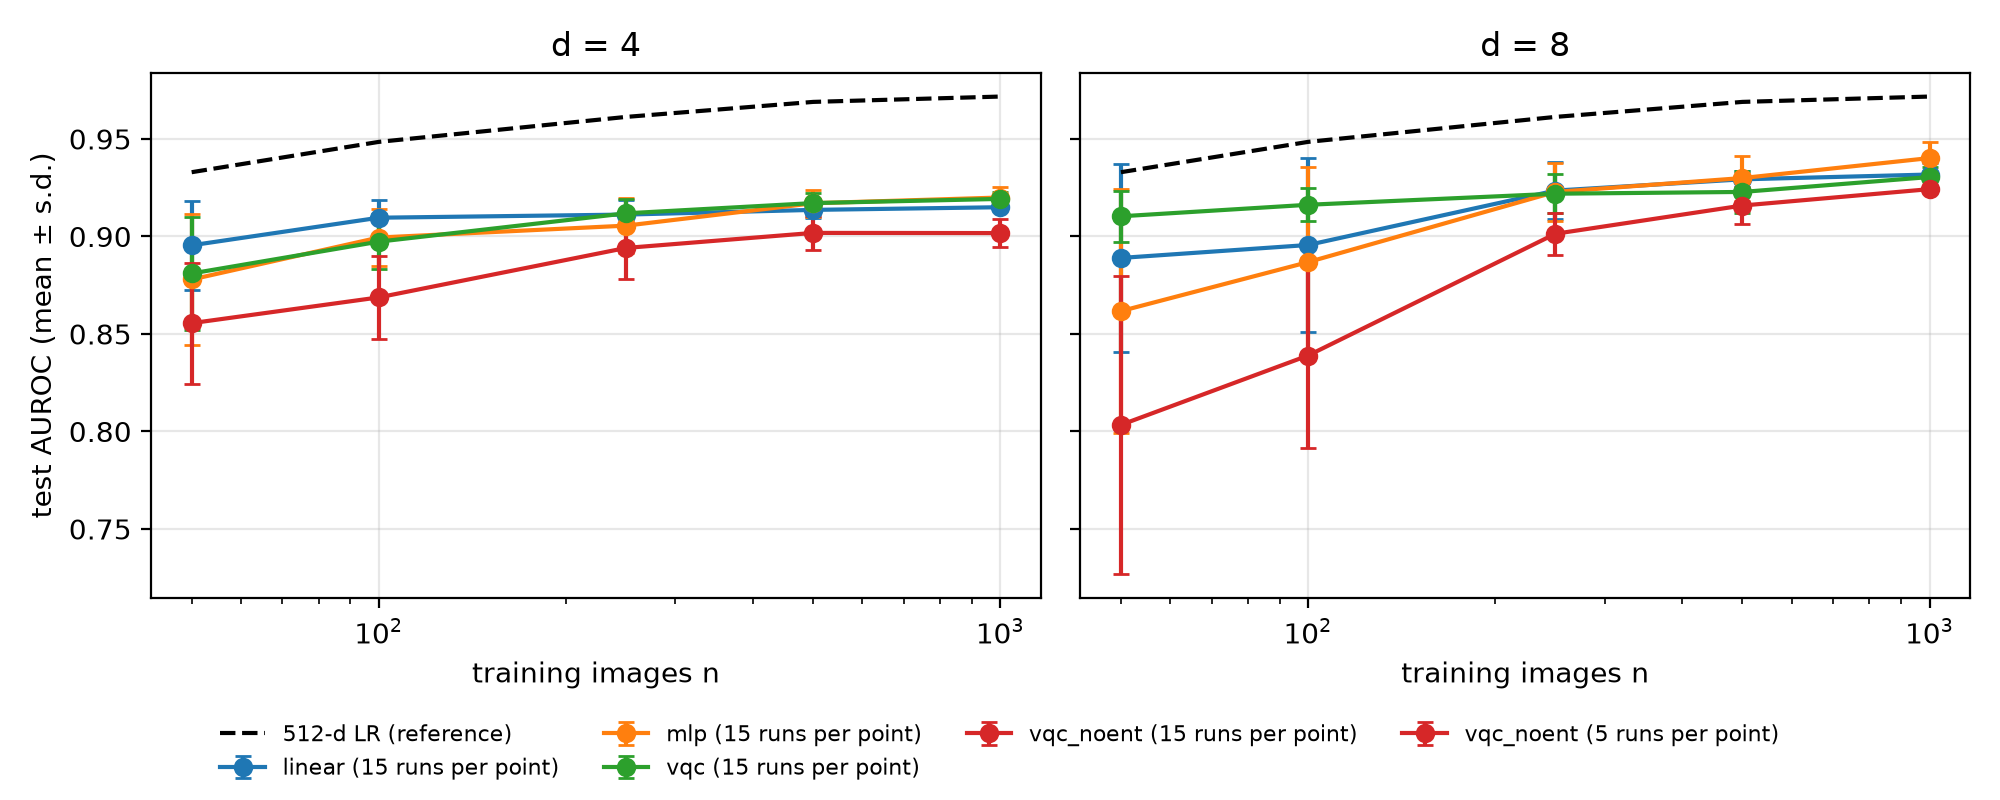
\includegraphics[width=\columnwidth]{../results/learning_curves.png}
\caption{Test AUROC versus training-set size $n$ at $d=4$ (left) and
$d=8$ (right). Dashed: logistic regression on all 512 features. Error bars:
s.d.\ over runs. $d=8$ VQC: 15 runs at $n\le100$, 13 at $n=250$, 5 above.}
\label{fig:curves}
\end{figure}

\subsection{VQC versus parameter-matched classical heads}
\emph{Pre-registered test, $d=4$.} The VQC and the parameter-matched MLP
are statistically equivalent at both small training sizes:
$\Delta=+0.003$ $[-0.008,+0.014]$ at $n=50$ and $\Delta=-0.002$
$[-0.009,+0.005]$ at $n=100$. Both intervals lie within the $\pm0.02$
equivalence margin. Neither lies entirely above zero, so \textbf{the
small-data hypothesis is falsified at $d=4$} (but see $d=8$ below). The
heads remain equivalent at every larger $n$. At $n=250$ the interval
$[+0.0004,+0.013]$ lies above zero but also inside the margin; we report
this as a statistically detectable but practically negligible difference,
and note that the pre-registered rules did not specify which label takes
precedence when both apply. The 5-parameter linear head outperforms the
VQC at $n=50$ ($\Delta=-0.014$ $[-0.024,-0.006]$); the VQC is slightly
ahead of it at $n\ge500$ ($\Delta=+0.004$ at $n=1000$).

\emph{Pre-registered test, $d=8$.} With 15 runs per point at $n\le100$,
the test is passed at $d=8$: $\Delta=+0.049$ $[+0.022,+0.077]$ at $n=50$
and $\Delta=+0.029$ $[+0.007,+0.054]$ at $n=100$. Three qualifications
apply. The subsample-level sensitivity check includes zero at $n=100$
($[-0.004,+0.072]$). Against the 9-parameter linear head the VQC's lead at
$n=50$ is inconclusive ($+0.021$ $[-0.001,+0.044]$). The lead vanishes by
$n=250$ ($+0.001$ $[-0.005,+0.008]$) and reverses at $n=1000$, where the
MLP is better ($-0.013$ $[-0.022,-0.004]$; one seed for $n\ge500$). The
effect is driven largely by stability: at $n=50$ the classical heads vary
with s.d.\ 0.048 (linear) and 0.063 (MLP) across runs, the VQC with 0.013.

\subsection{Entanglement ablation}
Removing all CNOT gates lowers test AUROC at every training size
(Table~\ref{tab:auroc4}). At $d=4$ the paired difference
$\Delta=\mathrm{AUROC}_{\mathrm{VQC}}-\mathrm{AUROC}_{\text{no CNOT}}$
ranges from $+0.015$ $[+0.013,+0.019]$ at $n=500$ to $+0.029$
$[+0.023,+0.034]$ at $n=100$. All intervals lie above zero, and the
subsample-level check agrees. At $d=8$ (one seed) the gain is larger:
$+0.104$ $[+0.050,+0.159]$ at $n=50$ and $+0.077$ $[+0.035,+0.120]$ at
$n=100$. Without entanglement the circuit's output is a sum of
single-feature functions, $f(\mathbf{x})=\sum_i g_i(x_i)$, so the gain
indicates that the entangled circuit uses interactions between features.
Both variants have the same number of parameters.

\subsection{Circuit depth}
Table~\ref{tab:depth} varies the number of layers $L$ at $d=4$. Three
layers outperform two by $+0.019$ $[+0.007,+0.031]$ at $n=50$ and by a
small positive margin at most larger $n$. A single layer is the most
stable at $n=50$ (s.d.\ 0.007) but levels off near 0.89 from $n=250$,
consistent with underfitting. The $L=3$ circuit exceeds the MLP at $n=50$
($+0.023$ $[+0.009,+0.038]$), but it is not parameter-matched (38 versus
25 parameters), the depth was selected after the fact, and it does not
exceed the linear head; we report it as exploratory.

\begin{table}[t]
\centering
\caption{Test AUROC versus circuit depth at $d=4$ (15 runs per point).}
\label{tab:depth}
\footnotesize
\begin{tabular}{@{}lccc@{}}
\toprule
$n$ & $L=1$ (14) & $L=2$ (26) & $L=3$ (38) \\
\midrule
50   & .898$\pm$.007 & .881$\pm$.029 & .900$\pm$.018 \\
100  & .901$\pm$.003 & .897$\pm$.014 & .908$\pm$.007 \\
250  & .887$\pm$.010 & .912$\pm$.008 & .917$\pm$.009 \\
500  & .891$\pm$.003 & .917$\pm$.005 & .919$\pm$.005 \\
1000 & .892$\pm$.008 & .919$\pm$.003 & .922$\pm$.003 \\
\bottomrule
\end{tabular}
\end{table}

\subsection{Noise}
Fig.~\ref{fig:noise} shows the VQC trained noiselessly at $n=1000$ and
evaluated under simulated noise (seed 0, 5 subsamples). Under depolarizing
gate noise alone, test AUROC is unchanged up to $p=0.03$ ($0.919$ at $p=0$
and $0.919$ at $p=0.03$). Balanced accuracy at the noiseless validation
threshold drops from $0.794$ to $0.620$ at $p=0.01$ and to $0.500$ at
$p=0.03$. Depolarizing noise shrinks every expectation value by the same
factor, $\langle Z\rangle\mapsto(1-4\lambda/3)\langle Z\rangle$ for a
channel of strength $\lambda$. This preserves the ranking of test images,
and with it AUROC, but moves all scores past the fixed threshold. With 2\%
readout error and 1024 shots added, AUROC stays within 0.012 of the
noiseless value up to $p=0.01$ and collapses to $0.574$ at $p=0.03$. At
that level the CNOT noise ($10p$) shrinks the signal to roughly a tenth of
its noiseless size, comparable to the shot noise. The CNOT-free circuit is
unaffected in AUROC under all conditions ($0.898$--$0.901$), because its
signal passes through no two-qubit gates. For the hardware run this
implies that the decision threshold should be recalibrated on hardware
outputs.

\begin{figure}[t]
\centering
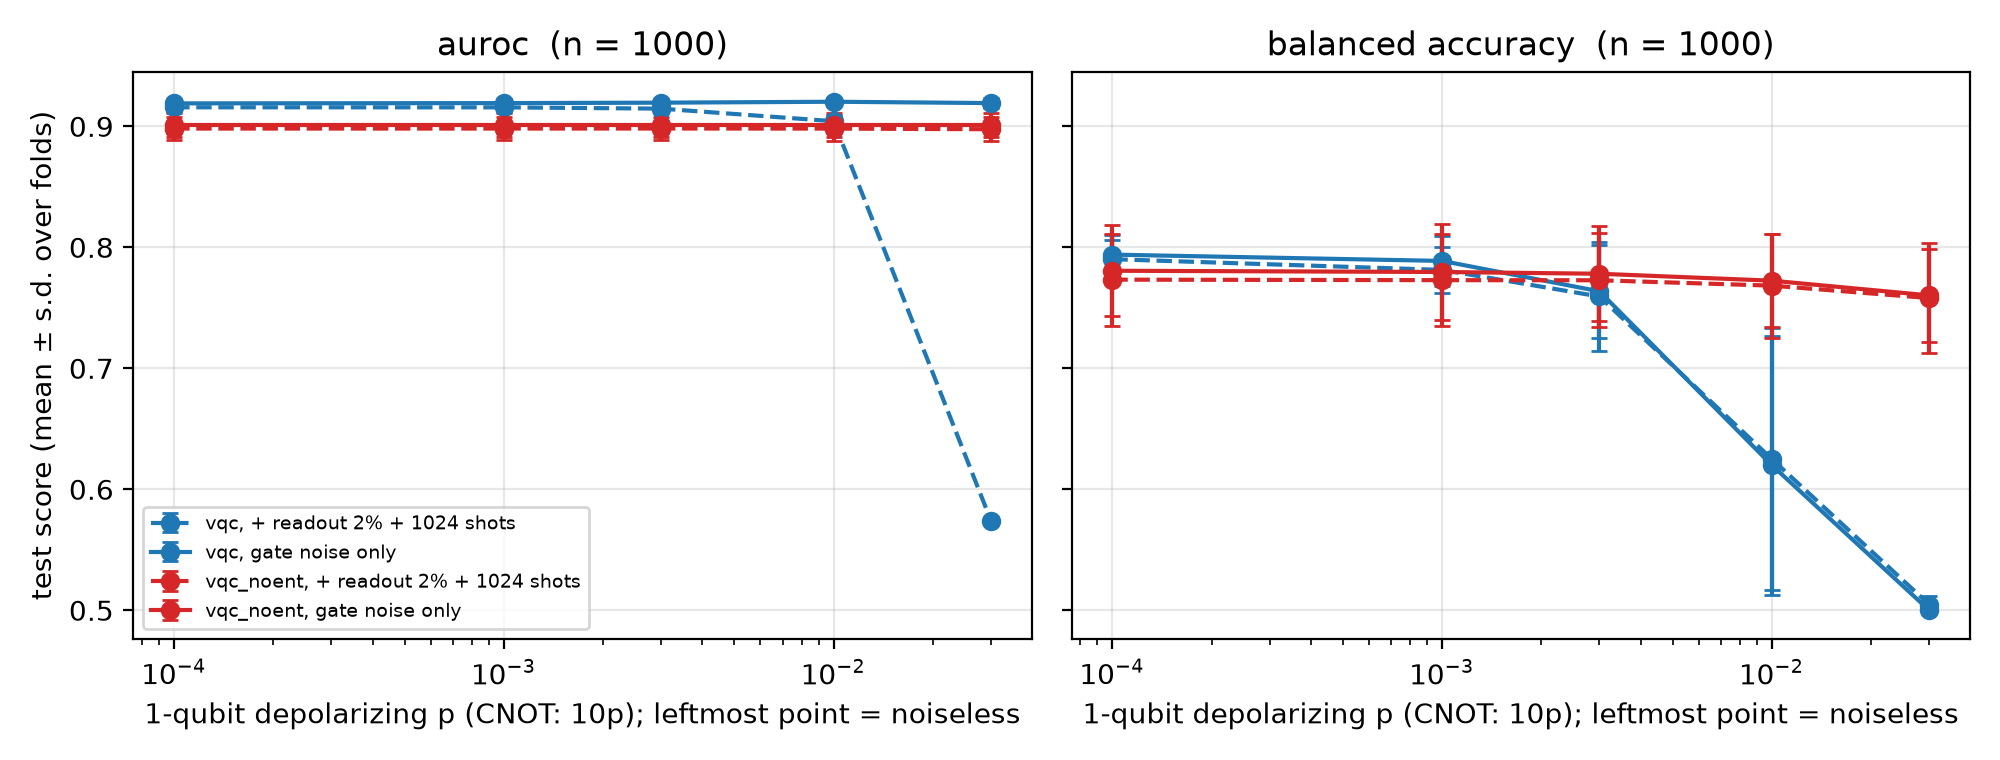
\includegraphics[width=\columnwidth]{../results/noise_sweep.png}
\caption{VQC heads trained noiselessly at $n=1000$, $d=4$, evaluated under
depolarizing noise $p$ on single-qubit gates and $10p$ on CNOTs.
Dashed: with 2\% readout error and 1024 shots. Mean $\pm$ s.d.\ over 5
subsamples (seed 0).}
\label{fig:noise}
\end{figure}

\begin{table}[t]
\centering
\caption{Circuit resources per input (from \texttt{qml.specs}).}
\label{tab:resources}
\footnotesize
\begin{tabular}{@{}lcccccc@{}}
\toprule
Circuit & Qubits & Params & Depth & 1q gates & CNOTs & Shots \\
\midrule
VQC, $d=4$         & 4 & 26 & 15 & 28 & 8  & exact / 1024 \\
VQC, $d=8$         & 8 & 50 & 23 & 56 & 16 & exact \\
No CNOT, $d=4$     & 4 & 26 & 7  & 28 & 0  & exact / 1024 \\
\bottomrule
\end{tabular}
\end{table}

% =====================================================================
\begin{thebibliography}{99}
\footnotesize
\bibitem{he2016} K.~He, X.~Zhang, S.~Ren, and J.~Sun, ``Deep residual learning for image recognition,'' in \emph{Proc. IEEE CVPR}, 2016, pp.~770--778.
\bibitem{cerezo2021} M.~Cerezo \emph{et al.}, ``Variational quantum algorithms,'' \emph{Nat. Rev. Phys.}, vol.~3, pp.~625--644, 2021.
\bibitem{mari2020} A.~Mari, T.~R. Bromley, J.~Izaac, M.~Schuld, and N.~Killoran, ``Transfer learning in hybrid classical-quantum neural networks,'' \emph{Quantum}, vol.~4, p.~340, 2020, doi: 10.22331/q-2020-10-09-340.
\bibitem{shahjalal2025} Shahjalal, J.~K. Fahim, P.~C. Paul, M.~R. Hossain, M.~T. Ahmed, and D.~Chakraborty, ``HQCNN: A hybrid quantum-classical neural network for medical image classification,'' arXiv:2509.14277, 2025.
\bibitem{singh2025} G.~Singh, H.~Jin, and K.~M. Merz, Jr., ``Benchmarking MedMNIST dataset on real quantum hardware,'' arXiv:2502.13056, 2025.
\bibitem{bowles2024} J.~Bowles, S.~Ahmed, and M.~Schuld, ``Better than classical? The subtle art of benchmarking quantum machine learning models,'' arXiv:2403.07059, 2024.
\bibitem{kolle2024} M.~K\"olle, J.~Maurer, P.~Altmann, L.~S\"unkel, J.~Stein, and C.~Linnhoff-Popien, ``Disentangling quantum and classical contributions in hybrid quantum machine learning architectures,'' in \emph{Proc. 16th Int. Conf. Agents and Artificial Intelligence (ICAART)}, vol.~3, 2024, pp.~649--656, doi: 10.5220/0012381600003636.
\bibitem{schuldkilloran2022} M.~Schuld and N.~Killoran, ``Is quantum advantage the right goal for quantum machine learning?'' \emph{PRX Quantum}, vol.~3, p.~030101, 2022.
\bibitem{martinperez2026} D.~Mart\'{\i}n-P\'erez, F.~Rodr\'{\i}guez-D\'{\i}az, D.~Guti\'errez-Avil\'es, A.~Troncoso, and F.~Mart\'{\i}nez-\'Alvarez, ``Hybrid classical-quantum transfer learning with noisy quantum circuits,'' \emph{Comput. Model. Eng. Sci.}, 2026, doi: 10.32604/cmes.2026.082712, arXiv:2603.16973.
\bibitem{yang2023} J.~Yang \emph{et al.}, ``MedMNIST v2 -- A large-scale lightweight benchmark for 2D and 3D biomedical image classification,'' \emph{Sci. Data}, vol.~10, p.~41, 2023.
\bibitem{kermany2018} D.~S. Kermany \emph{et al.}, ``Identifying medical diagnoses and treatable diseases by image-based deep learning,'' \emph{Cell}, vol.~172, no.~5, pp.~1122--1131, 2018.
\bibitem{mcclean2018} J.~R. McClean, S.~Boixo, V.~N. Smelyanskiy, R.~Babbush, and H.~Neven, ``Barren plateaus in quantum neural network training landscapes,'' \emph{Nat. Commun.}, vol.~9, p.~4812, 2018.
\bibitem{bergholm2018} V.~Bergholm \emph{et al.}, ``PennyLane: Automatic differentiation of hybrid quantum-classical computations,'' arXiv:1811.04968, 2018.
\bibitem{kingma2015} D.~P. Kingma and J.~Ba, ``Adam: A method for stochastic optimization,'' in \emph{Proc. ICLR}, 2015.
\bibitem{mitarai2018} K.~Mitarai, M.~Negoro, M.~Kitagawa, and K.~Fujii, ``Quantum circuit learning,'' \emph{Phys. Rev. A}, vol.~98, p.~032309, 2018.
\bibitem{schuld2019} M.~Schuld, V.~Bergholm, C.~Gogolin, J.~Izaac, and N.~Killoran, ``Evaluating analytic gradients on quantum hardware,'' \emph{Phys. Rev. A}, vol.~99, p.~032331, 2019.
\bibitem{youden1950} W.~J. Youden, ``Index for rating diagnostic tests,'' \emph{Cancer}, vol.~3, no.~1, pp.~32--35, 1950.
\end{thebibliography}

\end{document}
